\documentclass[]{article}
\usepackage{amsmath}
\usepackage{fancyhdr}
\linespread{1.5}
\usepackage{subcaption}
\usepackage{tikz-qtree}
\usepackage{mathtools}
\usepackage[headsep=1cm, top=1.58cm,bottom=1cm,right=1.5cm,left=1.5cm]{geometry}
\usepackage[utf8]{inputenc}
\usepackage{lmodern, textcomp}
\usetikzlibrary{shapes,arrows.meta,positioning,bending}
\tikzset{every tree node/.style={minimum width=2em,draw,circle},
     blank/.style={draw=none},
     edge from parent/.style=
     {draw, edge from parent path={(\tikzparentnode) -- (\tikzchildnode)}},
     level distance=1.5cm}



\tikzstyle{process} = [rectangle,rounded corners,minimum width=3cm, minimum height=1cm, text centered, draw=black, fill=orange!15]

\tikzstyle{decision} = [diamond,aspect=2, minimum width=3cm, minimum height=1cm, text centered, draw=black, fill=pink]

\tikzstyle{arrow} = [thick,->,>=stealth]
\pagestyle{fancy}
\fancyhf{}
\usepackage{graphicx}
\usepackage{hyperref}
\usepackage{xepersian}
\settextfont{Yas}
\author{پارسا پورسیستانی-۹۹۱۳۰۳۶}

\newcommand{\gu}[1]{«#1»}
\headheight 75pt
\begin{document}
\begin{titlepage}
\newcommand{\HRule}{\rule{\linewidth}{0.5mm}} 

\center 


\includegraphics[scale=0.15]{logo2.png}\\[1cm]
\textsc{\LARGE \bfseries دانشکده ریاضی و علوم‌کامپیوتر}\\[0.7cm] 
\textsc{\Large \bfseries تمرین تحویلی لتک}\\[0.5cm] 
\HRule \\[0.4cm]
{ \huge \bfseries نرم‌افزار ریاضی}\\[0.4cm]
\HRule \\[1cm]
\textsc{\LARGE \bfseries پارسا پورسیستانی-۹۹۱۳۰۳۶}\\[0.7cm]
\today
\end{titlepage}
\newpage
\rhead{
	
\includegraphics[height=25mm]{logo.png}
	}
\lhead{
	\textsc{\large \bfseries  تمرین لتک}
}
\chead{
	\textsc{\large \bfseries  نرم‌افزار ریاضی}
}
  
\section*{سوال ۱.}
لورم ایپسوم متن ساختگی با تولید سادگی نامفهوم از صنعت چاپ، و با استفاده از طراحان گرافیک است، چاپگرها و متون بلکه روزنامه و مجله در ستون و سطرآنچنان که لازم است، و برای شرایط فعلی تکنولوژی مورد نیاز، و کاربردهای متنوع با هدف بهبود ابزارهای کاربردی می باشد، کتابهای زیادی در شصت و سه درصد گذشته حال و آینده، شناخت فراوان جامعه و متخصصان را می طلبد، تا با نرم افزارها شناخت بیشتری را برای طراحان رایانه ای علی الخصوص طراحان خلاقی، و فرهنگ پیشرو در زبان فارسی ایجاد کرد، در این صورت می توان امید داشت که تمام و دشواری موجود در ارائه راهکارها، و شرایط سخت تایپ به پایان رسد و زمان مورد نیاز شامل حروفچینی دستاوردهای اصلی، و جوابگوی سوالات پیوسته اهل دنیای موجود طراحی اساسا مورد استفاده قرار گیرد.
  \begin{center}
    \begin{tabular}{|c|c|c|}
    \hline
         نام & پریسا & توکلی \\
    \hline

رشته &
\multicolumn{2}{|c|}{علوم‌کامپیوتر}
\\
\hline
         شغل & دانشجو & کارشناسی \\
    \hline 
    
    شماره تماس &
\multicolumn{2}{|c|}{09999999999}
\\
\hline
    
    \end{tabular}
  \end{center}
\begin{center}
\end{center}
\newpage
\section*{سوال ۲.}
ضرب خارجی:\\
\begin{flushleft}
$
u = u_1i + u_2j+u_3k $
\\
$
v = v_1i + v_2j +v_3k
$
\\
$
u \times v = det 
\begin{pmatrix}
i & j & k\\
u_1& u_2 & u_3\\
v_1 & v_2 & v_3
\end{pmatrix} = 
(u_2v_3 - u_3v_2)i + (u_3v_1 - u_1v_3)j + (u_1v_2 - u_2v_1)k
$
\\
\end{flushleft}
خواص:
\begin{flushleft}
$ 
1) u \cdots (u \times v) = v \cdots (u \times v) = 0 $
\\

(مساحت متوازی‌الاضلاع تولید شده توسط u و v )
$
2) \lvert u \times v \rvert = |u||v| \sin \theta 
$

\[\bot u ,  v  \iff \ u \times v = 0 \]
\end{flushleft}
\newpage

\section*{سوال ۳.}
\begin{figure}[!ht]
\centering
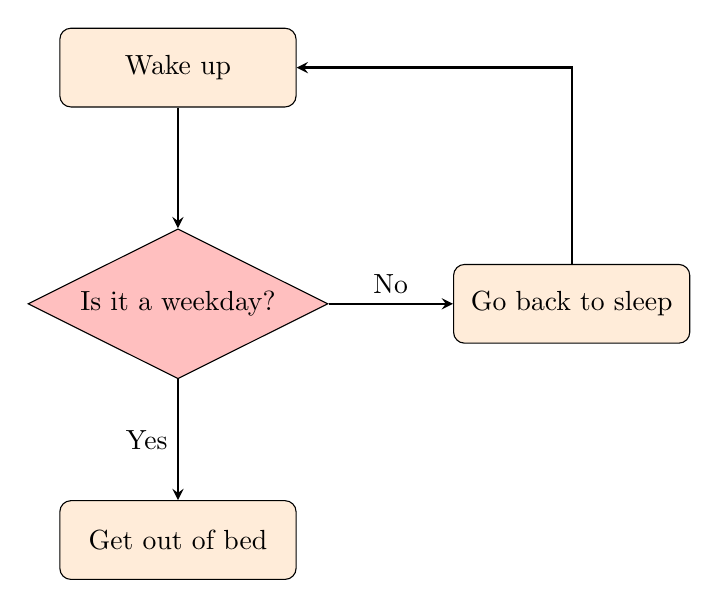
\begin{tikzpicture}[node distance=3cm]

\node (start) [process] {Wake up};

\node (d1) [decision,below of=start,yshift=0cm] {Is it a weekday?};

\node (d2) [process, below of=d1,yshift=0cm] {Get out of bed};

\node (r1) [process, right of=d1,xshift=2cm] {Go back to sleep};

\draw [arrow] (start) -- (d1);
\draw [arrow] (r1) |- (start);

\draw [arrow] (d1) -- node[anchor=east] {Yes} (d2);
\draw [arrow] (d1) -- node[anchor=south] {No} (r1);
\end{tikzpicture}
\caption{فلوچارت}
\end{figure}

\bigskip
\bigskip
\bigskip
\bigskip
\begin{figure}[!ht]
\centering
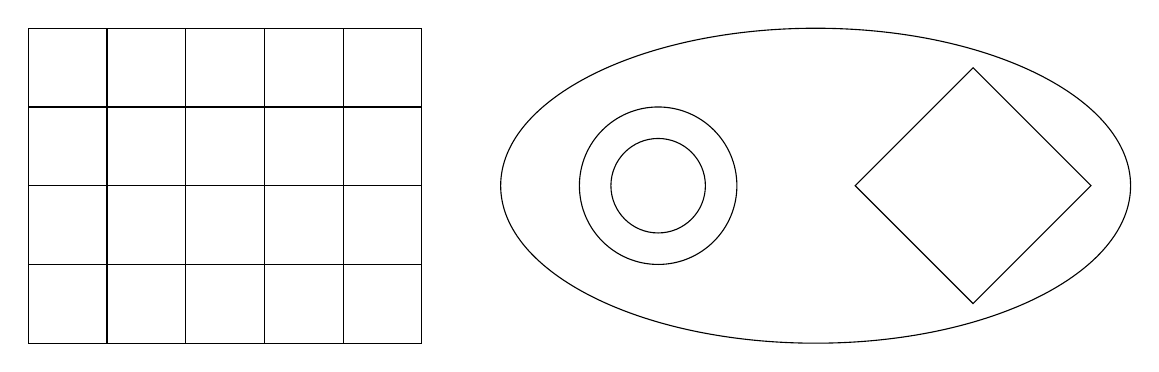
\begin{tikzpicture}[node distance=0cm]
\draw[step=1cm] (-5,-2) grid (0,2);

\draw(5,0) ellipse (4cm and 2cm);
\draw(3,0) circle (1cm);
\draw(3,0) circle (0.6cm);
\node [diamond,draw,minimum width=3cm,minimum height=3cm](d)  at (7,0){};
\end{tikzpicture}
\caption{دو تصویر}
\end{figure}
\end{document}